\section{Data pipelines}
\label{sec:pipelines}

This section describes the data pipelines we used for processing both curated and web data. Given the distinct nature and processing requirements of these two types of data, the pipelines are described in separate subsections.

\subsection{Pipeline for curated data}
\label{sec:pipelines.curated}

Curated datasets are published in a variety of formats and metadata. In contrast to web crawled data, these datasets consist of thematically related and high-quality texts, due to the previous curation process (e.g. reviewing for scientific articles). Therefore, a quality-based filter is less necessary and the preprocessing is based the pipeline in Figure \ref{fig:curated_pipeline}.

\begin{figure}[ht]
    \centering
    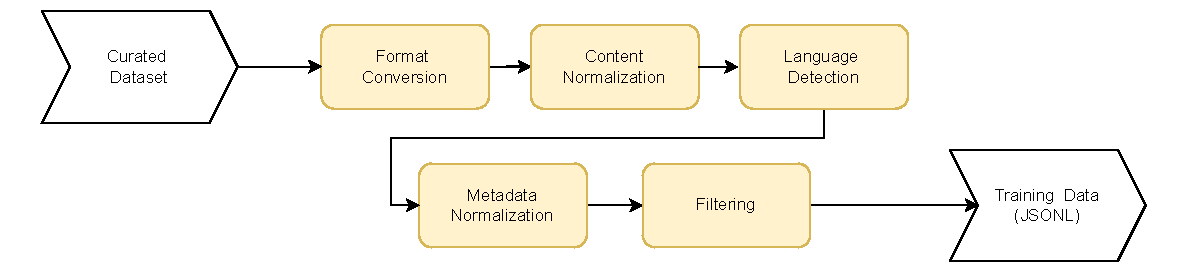
\includegraphics[width=\linewidth]{images/Curated_v4.drawio.pdf}
    \caption{\label{fig:curated_pipeline}%
    Data pipeline for curated datasets: The pipeline involves format conversion, content normalization, followed by language detection, content normalization and filtering. The output is high-quality training data in JSONL format.}
\end{figure}


\textbf{Format Conversion.}
The first step in processing curated data involves converting the raw data into JSONL format. Depending on the raw data's format, we employ different processing tools. For PDF documents, \textit{Grobid}\footnote{\url{https://github.com/kermitt2/grobid}} converts PDFs to XML/TEI as an intermediate format which we then convert to JSONL to identify and remove layout elements from the content. 
For Wikimedia datasets (e.g., Wikipedia, Wikibooks), \textit{wikiConverter} parses the Wikimedia XML dumps and converts them to JSONL. The data is first converted using \textit{mwparserfromhell}\footnote{\url{https://github.com/earwig/mwparserfromhell}}, then list pages and disambiguation pages are removed, and finally the remaining data is processed as with other curated datasets. 
For any other format (e.g. plain text, csv, sql dumps, etc), we created custom conversion tools.
%%DONEJL: unclear which parts of libraries we use and which parts we implemented

\subsubsection{Normalization}
\label{sec:pipelines.curated.normalization}
Normalizing the content is important to ensure that the rest of the pipeline consistently handles data, facilitating versioning, processing, and sharing. We implement two types of normalization: content normalization and metadata normalization.



\textbf{Content Normalization.}
Content normalization ensures that the text data is uniformly formatted and encoded. 
(i) All text data is encoded in UTF-8 to maintain a standard character encoding format.
(ii) We apply NFKC normalization\footnote{Normalization Form KC as described in \url{https://unicode.org/reports/tr15/##Norm_Forms}} to the text content, converting characters to their canonical decomposition followed by compatibility composition to ensure that visually similar characters are represented consistently.  
(iii) Excessive white space is trimmed, and inconsistent spacing is corrected. 
(iv) Finally, we remove common conversion artefacts such as HTML tags or special characters to ensure the text is free from noise. 


\textbf{Metadata Normalization.}
Metadata normalization is important to maintain a consistent set of essential metadata attributes that provide a snapshot of each document. This metadata forms the basis for subsequent analysis and filtering steps.
The format for a single document (a line in a JSONL file) is as follows:

\begin{verbatim}
{
    "meta": {
        "docid": <corpus/language/fileno/docno>,
        "url": <url:String>,
        "title": <title:String>,      
        "download_date": <ISO-date:String>",
        "language": <ISO-language-code:String>,
        "language_score": <language-detection-score:Float>},
    "text": <text:String>
}
\end{verbatim}
\noindent
Where
\begin{itemize}
\item \texttt{meta} contains all document metadata.
\item \texttt{docid} is a unique ID comprised of the corpus name, the number of the file a document originates from, and the running document number within this file.
\item \texttt{url} is a string representing the URL of a document (where appropriate).
\item \texttt{title} is the title of a document (where appropriate).
\item \texttt{download\_date} is the download date in YYYY-MM-DD format.
\item \texttt{language} is a 2- or 3-letter ISO language code \cite{iso639} for the language of the content.
\item \texttt{language\_score} is a score estimated from language detection \cite{joulin_grave_etal2016a} (1.0 where the language is not ambiguous); ``xx'' is used for non-language content such as source code.
\item \texttt{text} is the normalized document content. 
\end{itemize}
For an example document, see Appendix \ref{ssec:appendix.metadataexample}.
Note that the example for the document format 
%%DONE \todo[inline]{Appendix example?} 
already includes information from language detection.

\subsubsection{Language Detection}
\label{sec:pipelines.curated.langdetect}

Following content normalization, language identification is performed using \textit{fasttext} \cite{joulin_grave_etal2016a}. The detected language code is included both in the metadata field and as part of the filename for the pipeline output to enable grouping of data by language. %During this process, documents with mixed-language content, noise, or under-resourced languages (e.g., Dutch and Afrikaans) may receive lower language scores. 

\subsubsection{Filtering}
\label{sssec:pipelines.curated.prefiltering}

To ensure appropriate data quality, we aim to remove low-quality documents as early as possible in the processing pipeline. 

We apply a set of filters to remove some outliers:
\begin{itemize}
    \item Documents with a language score lower than 0.5 are filtered out.
    \item Documents that contain fewer than 200 characters are removed.
\end{itemize}

These thresholds (200 characters, 0.5 language score) were chosen based on settings used in previous projects (e.g., HPLT\footnote{\url{https://hplt-project.org/datasets/v1}}) and are designed to ensure that only relevant and high-quality data proceeds to the subsequent stages of processing.


The final output of the curated data pipeline is a set of JSONL files, organized by language and corpus, ready for further analysis and model training.


\subsection{Pipeline for web data}
\label{sec:pipelines.web}

\begin{figure}[ht]
    \centering
    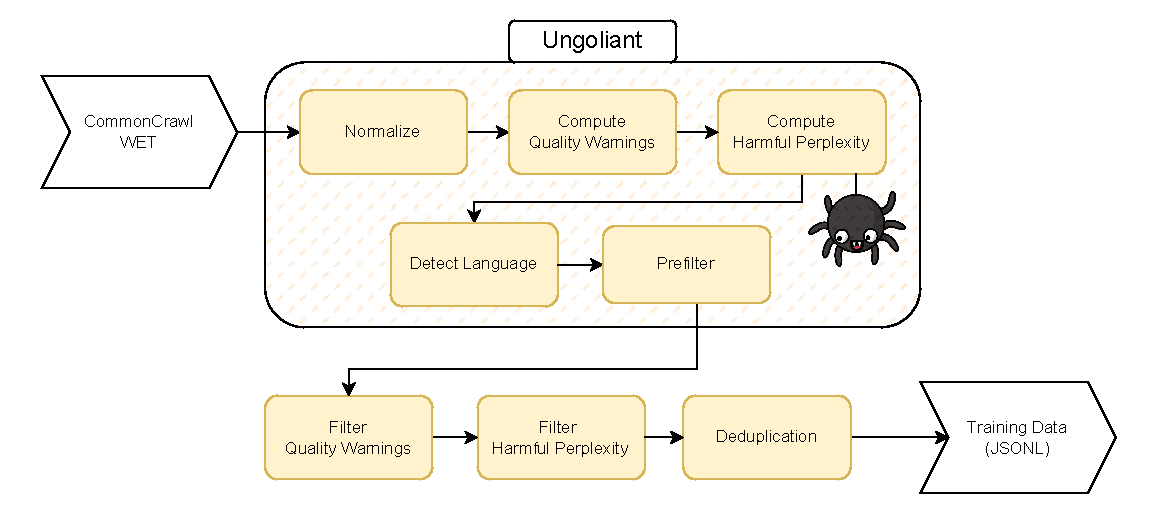
\includegraphics[width=\linewidth]{images/Webdata_v2.xml.drawio.pdf}
    \caption{\label{fig:web_data_pipeline}%
    Overview of the Web Data Processing Pipeline: The pipeline processes WET files with Ungoliant by normalizing, computing quality warnings and harmful-perplexity, detecting language, and prefiltering. Afterwards, data is filtered based on quality and harmful-perplexity before deduplication, producing high-quality training data in JSONL format.
   }
\end{figure}

Processing web data from large-scale sources like CommonCrawl presents significant challenges due to its unstructured and noisy nature. To transform this raw web data into a suitable format for training LLMs, we utilized a specialized pipeline (see Figure \ref{fig:web_data_pipeline}). This section provides a detailed breakdown of each processing stage, including normalization, filtering, and deduplication, using the Ungoliant pipeline.

\subsubsection{Dataset Acquisition and Preparation}
\label{sec:pipelines.web.prep}

The process begins by downloading CommonCrawl dumps in WET file format using a custom download script. These dumps contain the textual content and metadata of web pages, compressed in \texttt{.txt.gzip} format. After retrieving the raw data, we organized it into separate folders based on the dump year for easier processing.


\subsubsection{Ungoliant Pipeline}
\label{sec:pipelines.web.ung}

The core of the web data processing relies on the Ungoliant pipeline \cite{abadji_suarez_etal2021}, a modular system optimized for handling CommonCrawl corpora and producing an OSCAR-like dataset \cite{abadji_suarez_etal2022}. The Ungoliant pipeline is conceptually split into several key components:

\begin{itemize}
    \item \textbf{Normalization}: Similar to the normalization applied to curated data (see Section \ref{sec:pipelines.curated}), this step ensures consistency in text encoding, removing noise, normalizing text formatting, and encoding all content into UTF-8.
    \item \textbf{Computation of quality warnings}: Ungoliant generates quality warnings for each document which are then used for subsequent filtering stages.
    \item \textbf{Computation of harmful-perplexity}: Harmful content is identified using perplexity scores based on a pretrained KenLM model \cite{jansen_tong_etal2022}. This model evaluates documents to determine whether they contain harmful content (e.g., adult material).
    \item \textbf{Language detection}: Sentence-based language identification is performed using embedded\footnote{Ungoliant supports the detection of 176 languages. } pretrained fastText models \cite{joulin_grave_etal2016a,joulin_grave_etal2016b}. 
    \item \textbf{Prefiltering}: Documents are filtered based on criteria similar to those used for curated data (see Section \ref{sssec:pipelines.curated.prefiltering}), such as removing documents with a low number of characters or low language detection scores.
\end{itemize}


\subsubsection{Filtering}
\label{sec:pipelines.web.filtering}

After the documents pass through the Ungoliant pipeline, we apply additional filtering steps based on quality warnings and harmful-perplexity scores to further refine the dataset.


\textbf{Quality Warning filtering.} Ungoliant flags documents with several quality warnings: \texttt{tiny}, \texttt{noisy}, \texttt{header}, \texttt{footer}, and \texttt{short\_sentences}. These warnings are accompanied by predefined thresholds, and documents that exceed these thresholds are filtered out. The thresholds are defined as follows:
 \begin{itemize}
     \item \texttt{tiny}: When the document contains fewer than 5 sentences (lines).
     \item \texttt{noisy}:  When the ratio of non-letters to the total number of characters exceeds 50\%.
     \item \texttt{header}: Defined through a three-step process:
     \begin{itemize}
        \item Iterate through the first 20\% of a document\footnote{The percentage is calculated on a line-base,  i.e. when the character '$\backslash n$' is found.}. 
         \item Identify short sentences (lines) with fewer than 100 characters.
         \item Annotate the document as \texttt{header} if more than 50\% of the sentences in this section are short.

     \end{itemize}
     \item \texttt{footer}: Similar to the header but applied in reverse order to the above one.

     \item \texttt{short\_sentences}: When the document has a high number ($\ge 50\%$) of lines with less than 100 characters. 
 \end{itemize}

\textbf{Harmful-Perplexity Filtering.}
%source code here:https://github.com/oscar-project/ungoliant/blob/main/src/transformers/category.rs
Filtering adult content is a critical part of ensuring that the models are trained on safe and appropriate data. We use the perplexity scores provided by the KenLM-based model trained on adult content from the UT1 Blacklist \cite{jansen_tong_etal2022} as part of the Ungoliant pipeline. Lower perplexity scores indicate a higher likelihood that the document contains harmful or adult content. We set a perplexity threshold of 5, meaning any document with a perplexity score below this threshold is filtered out.


\subsubsection{Document deduplication}
\label{sec:pipelines.web.dedup}


Building on the quality filtering performed in the previous stage, the next step after running the Ungoliant pipeline is document deduplication. This process refines the dataset by removing both exact and near duplicate documents, thus reducing the overall size of the data and improving its quality for LLM training.
After extensive testing \cite{leveling_helmer_etal2024}, we found that the MinHash/LSH algorithm offers the best balance of precision, recall, and computational efficiency for deduplicating large volumes of web data. The deduplication process was executed on a per-dump and per-language basis (``local'' deduplication), which is both convenient and backed by newer research \cite{penedo_kydlicek_etal2024} that confirms that \emph{local} deduplication is more favorable than \emph{global} (across dump and/or language) approaches for preserving data diversity while minimizing redundancy.


\subsection{Technical Infrastructure}
\label{sec:pipelines.infrastructure}

To  effectively manage the extensive data processing requirements, we leveraged significant computational resources. The processing of large-scale datasets, including both curated datasets and CommonCrawl data, required the use of high-performance computing infrastructure.

Initially, a NVIDIA DGX-2 machine was employed for downloading and processing the curated datasets, as well as for deduplicating the first CommonCrawl dumps. As the volume of data increased, the processing of the remaining CommonCrawl datasets was distributed across two large compute clusters.

The technical specifications of these compute clusters are as follows:

\begin{itemize}
    \item Compute Cluster 1: Provided by TU Dresden, consisting of compute nodes with 2 x Intel Xeon Platinum 8470 (52 cores) @ 2.00 GHz CPU and 512 GB RAM.
    \item Compute Cluster 2: Provided by FZ Jülich, consisting of compute nodes with 2 x Intel Xeon Platinum 8168 (2x24 cores) @ 2.7 GHz CPU and 192 GB RAM.
\end{itemize}

These resources enabled us to handle the extensive data processing requirements necessary for pretraining our large language models.



